\documentclass[aspectratio=169,11pt]{beamer}
\usetheme{Boadilla}
\usecolortheme{seahorse}
\setbeamertemplate{navigation symbols}{}
\usefonttheme{professionalfonts}
\usepackage{booktabs}
\usepackage{amsmath}
\usepackage{xcolor}
\definecolor{good}{HTML}{2E7D32}
\definecolor{bad}{HTML}{C0392B}
\definecolor{acc}{HTML}{2E86AB}
\setbeamercolor{frametitle}{bg=acc,fg=white}
\setbeamercolor{title}{fg=acc}
\setbeamercolor{structure}{fg=acc}
\newcommand{\dG}{\Delta_{\mathrm r}G^{\prime\circ}}
\newcommand{\good}[1]{\textcolor{good}{#1}}
\newcommand{\bad}[1]{\textcolor{bad}{#1}}

\title{QC/ML prediction of metabolite reaction $\dG$}
\subtitle{What works, what doesn't, and where QC actually helps}
\date{\today}
\author{ModelSEED thermodynamics --- discussion notes}

\begin{document}

\maketitle

\begin{frame}{The question, and the honest one-line answer}
  \textbf{Goal:} compute standard transformed reaction Gibbs energies $\dG$ for
  metabolic reactions accurately enough to (a) adjudicate dGPredictor vs.\
  experiment, and (b) cover ModelSEED at large ($\sim$48k reactions).

  \vspace{1em}
  \textbf{Method under test:} a physics-only composite
  \[
    G_{\mathrm{aq}} = \underbrace{E_{\text{MLIP}}(\text{gas})}_{\text{MACE-POLAR-1}}
      + \underbrace{\Delta G_{\text{solv}}(\text{ALPB})}_{\text{xtb GFN2}}
      + \underbrace{G_{\text{RRHO}}}_{\text{xtb}}
    \;\rightarrow\; \text{Alberty transform to pH 7}
  \]

  \vspace{1em}
  \begin{alertblock}{Bottom line}
  On measured chemistry the data-driven methods already win
  (\good{eQuilibrator 3.0 kJ/mol}); the physics composite is at \bad{36 kJ/mol}
  and \emph{cannot be calibrated into competitiveness}. But QC has three narrow,
  defensible niches --- and the failure is a specific, quantified one.
  \end{alertblock}
\end{frame}

\begin{frame}{Where we started: the 10 top-disagreement reactions}
  \begin{columns}
    \begin{column}{0.54\textwidth}
      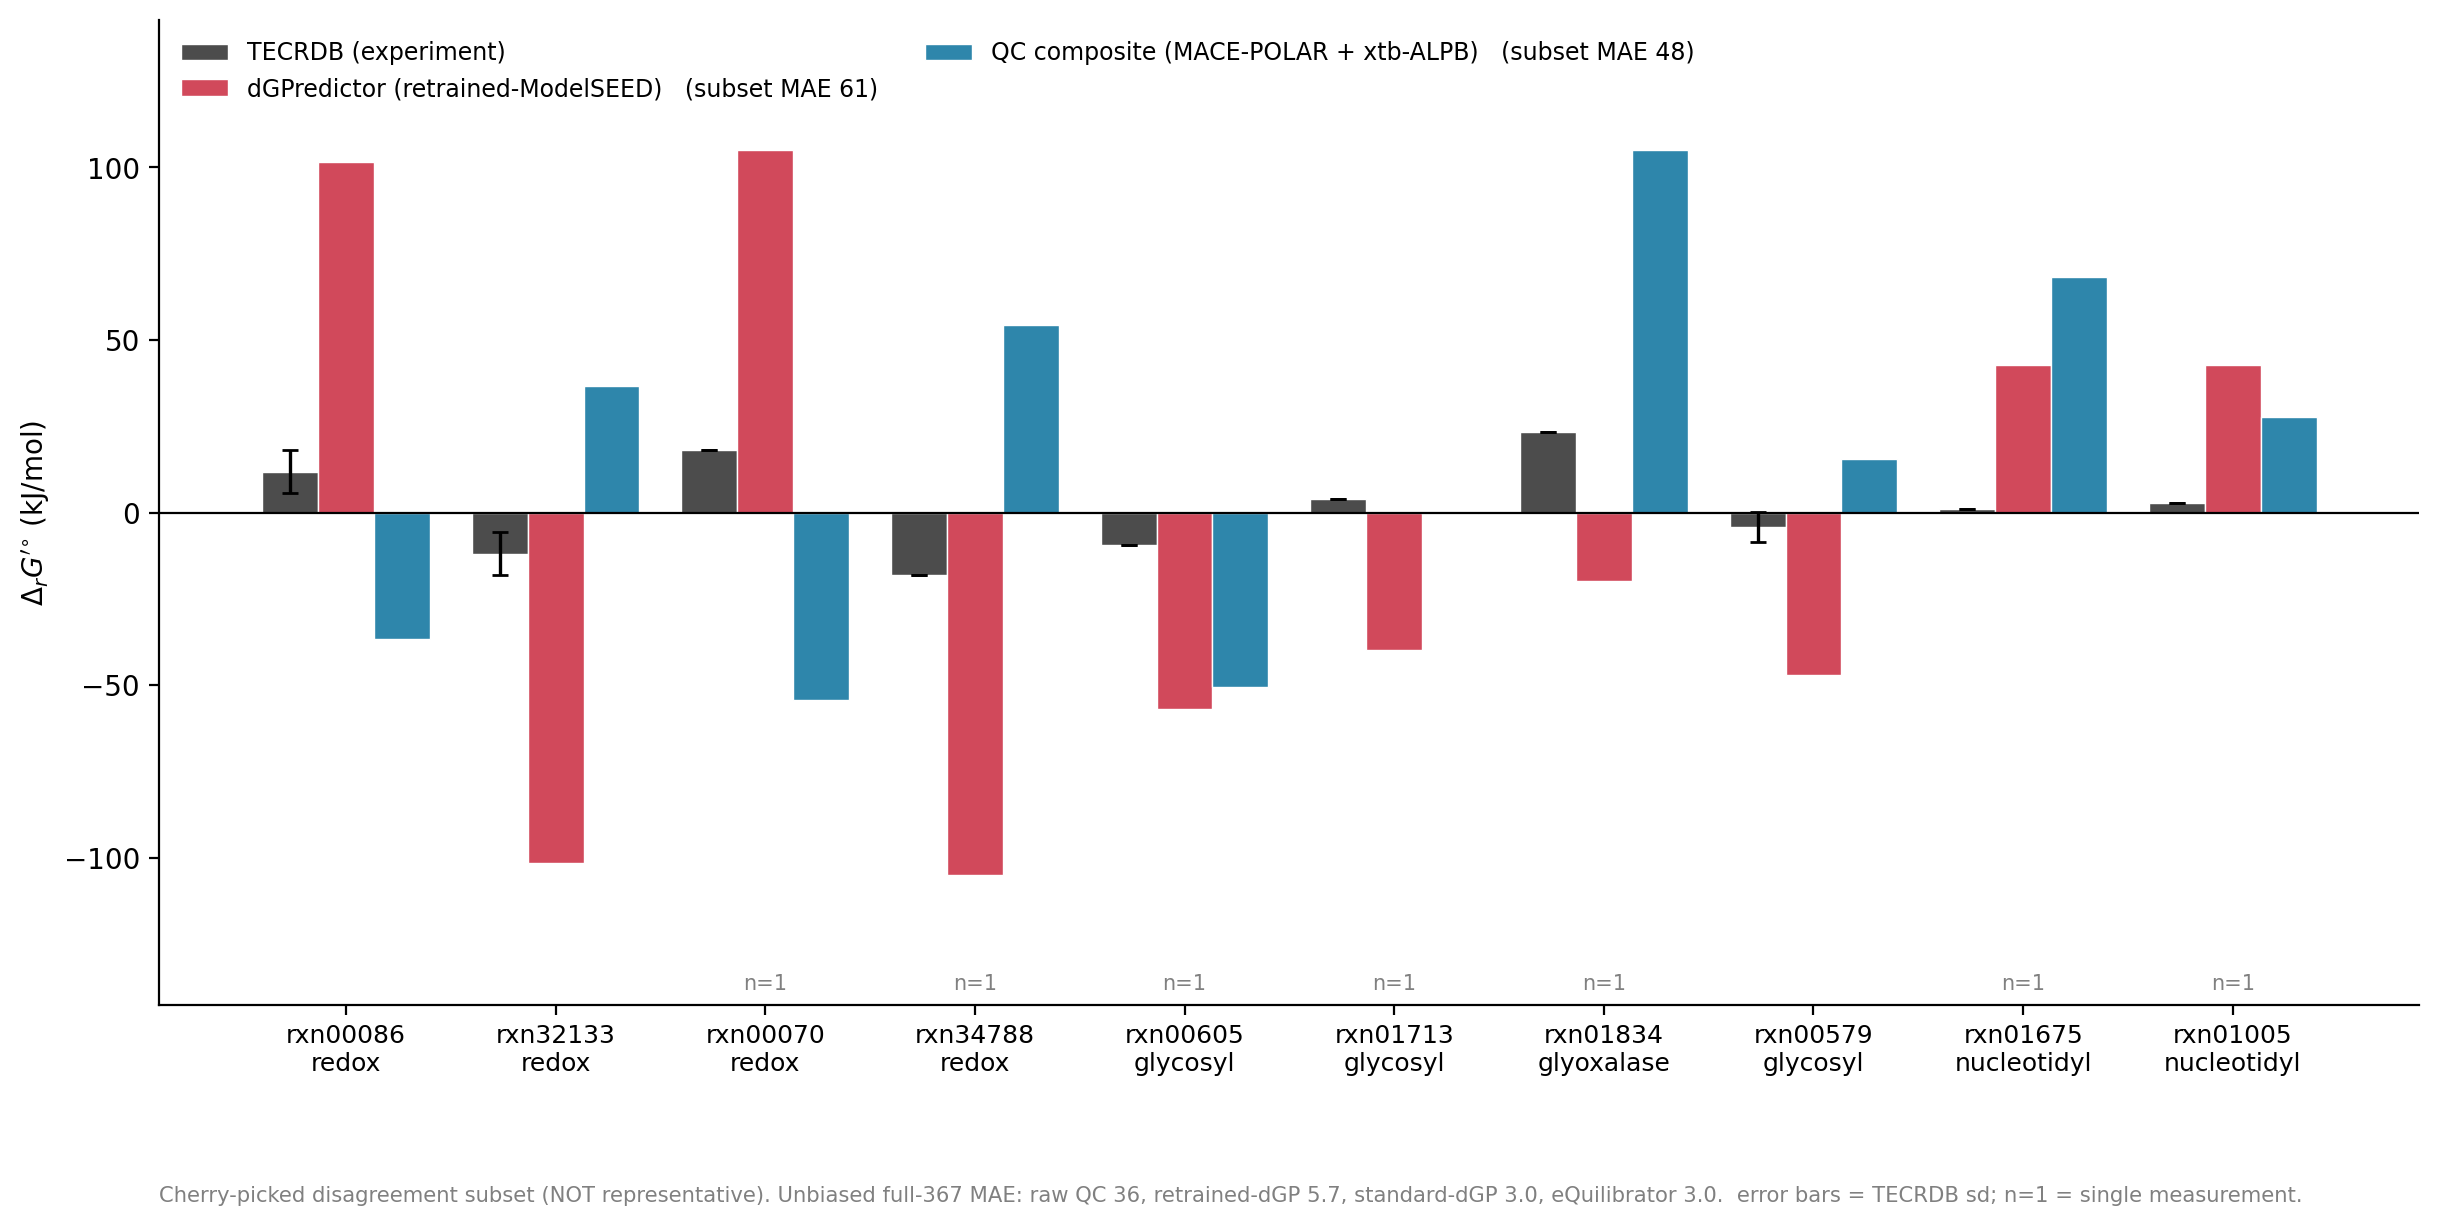
\includegraphics[width=\linewidth]{figures/top10.png}
    \end{column}
    \begin{column}{0.44\textwidth}
      \small
      \begin{tabular}{lr r}
        \toprule
        method & MAE & signs \\
        \midrule
        eQuilibrator & \good{3.6} & --- \\
        predict-zero & 10.5 & --- \\
        \textbf{QC + ext.\ refs} & \textbf{16.1} & \textbf{10/10} \\
        QC composite & 31.7 & 7/10 \\
        dGPredictor & 61.2 & 8/10 \\
        \bottomrule
      \end{tabular}

      \vspace{1em}
      Parameter-free external anchors (redox $E^{\circ\prime}$, isodesmic vs.\
      a measured pyrophosphorylase / sucrose phosphorylase) fix
      \emph{direction} 10/10 --- the adjudication-relevant property.
      \textbf{Still loses to predict-zero on MAE.}
    \end{column}
  \end{columns}
\end{frame}

\begin{frame}{Full TECRDB run: 367 reactions (80\% of all distinct reactions)}
  \begin{columns}
    \begin{column}{0.5\textwidth}
      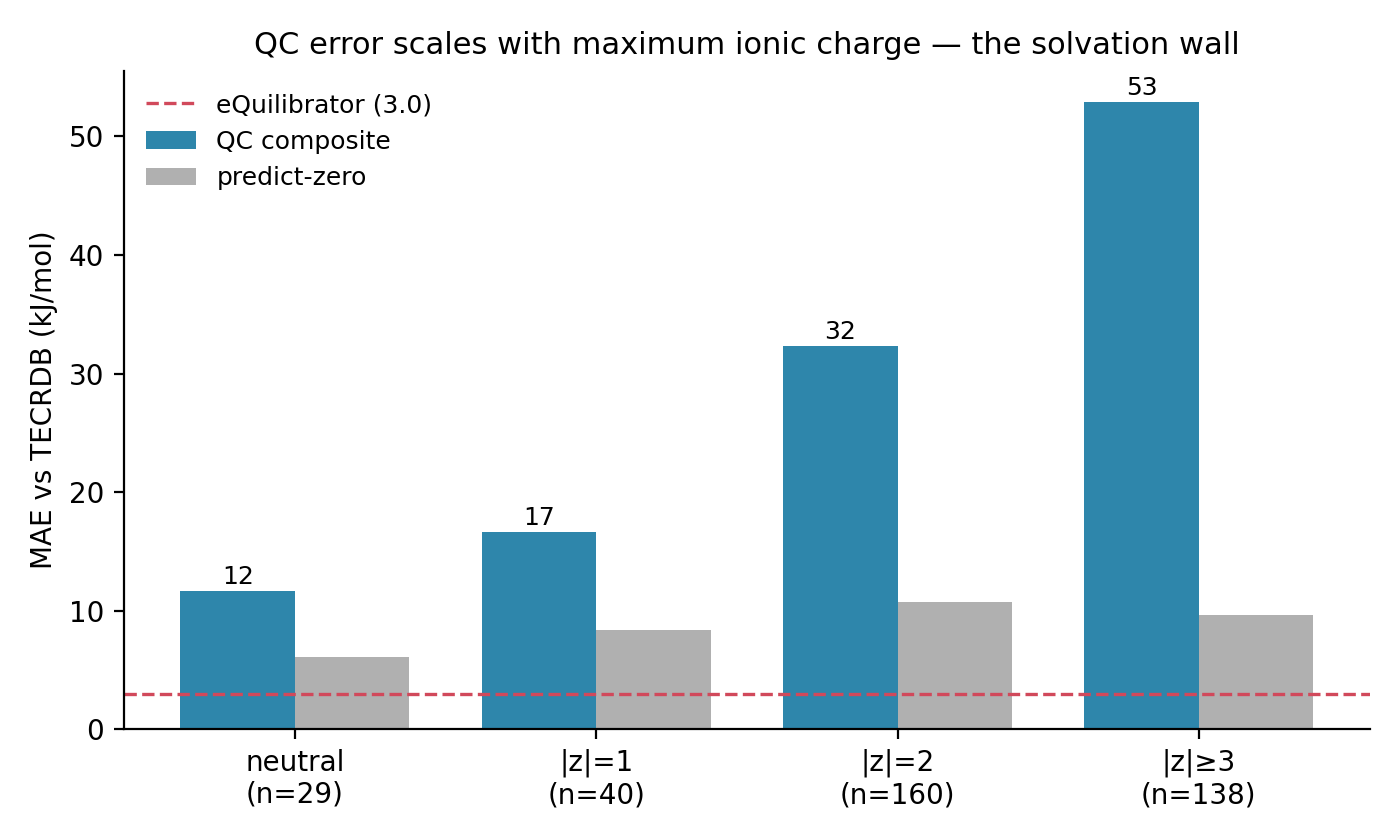
\includegraphics[width=\linewidth]{figures/charge_wall.png}
    \end{column}
    \begin{column}{0.5\textwidth}
      \begin{itemize}
        \item QC MAE \bad{36.1} vs predict-zero \good{9.7} vs eQuilibrator
          \good{3.0}
        \item Error is \textbf{monotone in ionic charge} $\Rightarrow$ it is
          \emph{solvation}, not the electronic method
        \item \textbf{No stratum beats predict-zero} --- not even neutral
          small molecules (11.6 vs 6.1)
      \end{itemize}
      \vspace{0.5em}
      \footnotesize
      453 compounds, 3\,263 conformers. CPU 21 min, GPU 2 min on
      80 cores / 8 GPUs.
    \end{column}
  \end{columns}
\end{frame}

\begin{frame}{The wall is phosphate solvation --- ruled out from every direction}
  \small
  \begin{tabular}{lll}
    \toprule
    lever tested & result & verdict \\
    \midrule
    electronic method (r2SCAN-3c vs MLIP) & 14.9 $\to$ 17.3 & not the cause \\
    MLIP choice (UMA vs MACE-POLAR)       & $r=0.98$ & not the cause \\
    geometry method (g-xTB vs GFN2 vs DFT) & net $<$1 kJ (terms cancel) & not the cause \\
    conformer sampling                    & error $\perp$ size & not the cause \\
    Mg$^{2+}$ speciation                  & +0.3 kJ net & not the cause \\
    CPCM-X solvation                      & phosphate $-150$ kJ & \bad{worse} \\
    explicit-water clusters               & over-stabilise polyanions & \bad{worse} \\
    explicit-solvent FEP                  & GPU-months & \bad{infeasible} \\
    \bottomrule
  \end{tabular}
  \vspace{1em}

  \begin{block}{Best achievable phosphate solvation, methods in hand}
    phenol 8.1 \quad thiol 17.9 \quad carboxylate 15.9 \quad
    \textbf{phosphate \bad{23.9} (ALPB, least bad)}
  \end{block}
  Phosphate is the most frequent charged group and no available continuum or
  cheap-cluster method gets it under $\sim$24 kJ/mol.
\end{frame}

\begin{frame}{The one replicated physical result: the phosphoanhydride bias}
  \begin{columns}
    \begin{column}{0.55\textwidth}
      \begin{itemize}
        \item Grouping by number of \textbf{P--O--P bonds cleaved}:
          \[
            \Delta(\text{P--O--P}) = -1:\quad
            \text{mean signed error } \bad{+63.8}\ \text{kJ}
          \]
        \item Pre-registered $+64\pm15$; replicated at $n{=}35$ (was 13),
          all same sign
        \item \textbf{Not geometry} (g-xTB test: net $<$1 kJ),
          \textbf{not electronic} --- it is the solvation of charge
          \emph{separation} when one polyphosphate becomes two anions
      \end{itemize}
    \end{column}
    \begin{column}{0.45\textwidth}
      \small
      \begin{tabular}{lrr}
        \toprule
        $\Delta$(P--O--P) & $n$ & mean signed \\
        \midrule
        $-2$ & 1  & $+169.7$ \\
        $-1$ & 35 & \bad{$+63.8$} \\
        $\phantom{-}0$ & 78 & $+12.0$ \\
        \bottomrule
      \end{tabular}
      \vspace{1em}

      A specific, quantified statement of \emph{where} continuum solvation
      fails. This is a publishable negative with an identified mechanism.
    \end{column}
  \end{columns}
\end{frame}

\begin{frame}{Does calibration rescue it? Across reactions yes --- across compounds no}
  \begin{columns}
    \begin{column}{0.5\textwidth}
      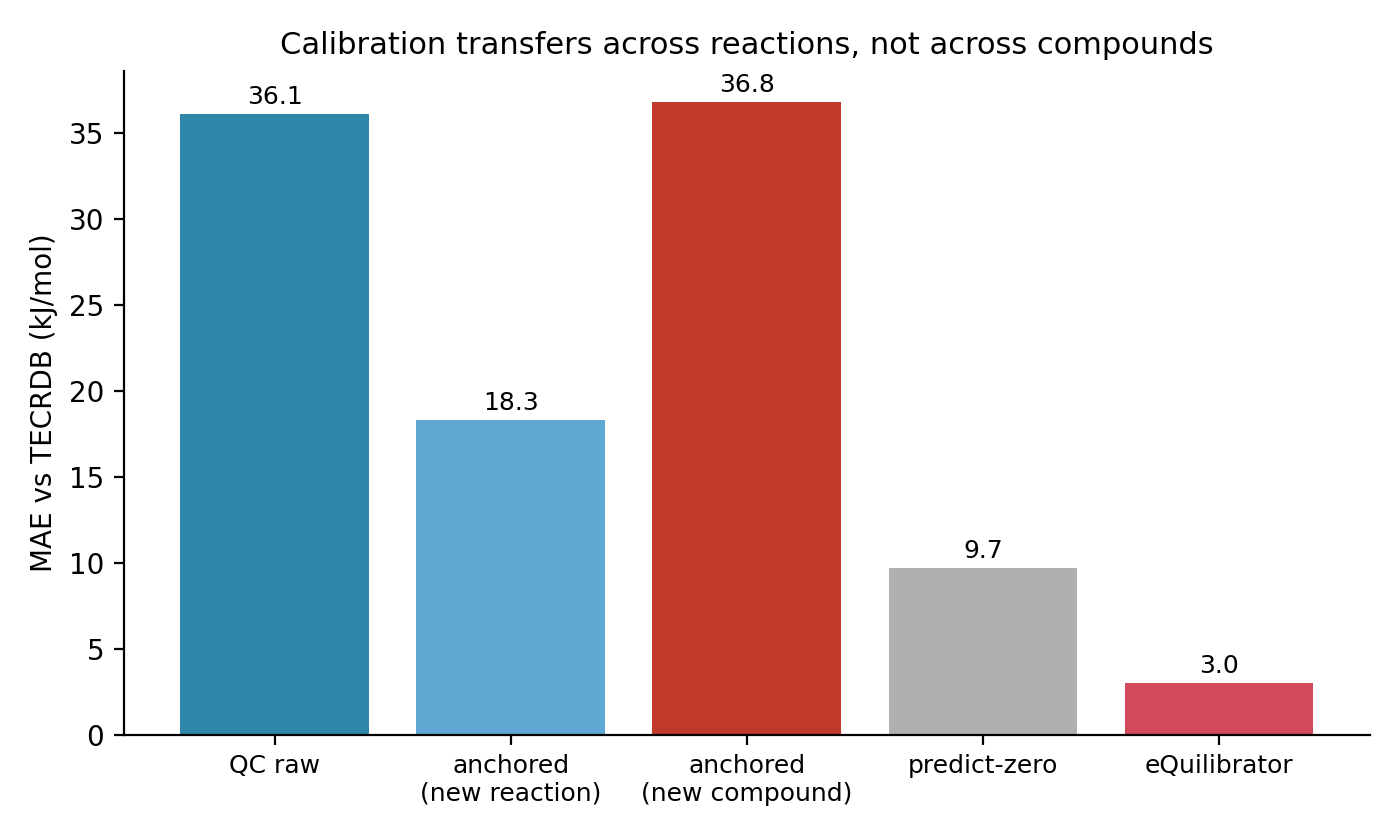
\includegraphics[width=\linewidth]{figures/calibration.png}
    \end{column}
    \begin{column}{0.5\textwidth}
      \begin{itemize}
        \item \textbf{New reaction, known species} (leave-reaction-out):
          $36.1 \to \good{18.3}$
        \item \textbf{New compound} (leave-compound-out):
          $36.1 \to \bad{36.8}$ --- \emph{no benefit}
        \item Decisive test: fitting the empirical model \emph{directly} to
          $\dG$ gives \good{7.8}; correcting QC gives 23.8; adding QC as a
          feature moves 7.8$\to$7.6 (\bad{$\sim$0.2 kJ})
      \end{itemize}
      \vspace{0.5em}
      \alert{Per-species anchoring is a lookup table over measured species, not
      a model.} The ModelSEED goal is exactly the \emph{unmeasured} compounds.
    \end{column}
  \end{columns}
\end{frame}

\begin{frame}{Data-driven baselines (full TECRDB, $n=364$)}
  \small
  \begin{tabular}{lrrrr}
    \toprule
    subset & QC & eQuilibrator & dGP standard & dGP retrained \\
    \midrule
    ALL & \bad{35.8} & \good{3.0} & \good{3.0} & 5.7 \\
    neutral $|z|{=}0$ & 11.6 & 0.6 & 0.7 & 0.7 \\
    $|z|{=}2$ & 32.4 & 2.9 & 3.0 & 5.5 \\
    $|z|{\geq}3$ & 50.5 & 4.0 & 3.7 & 7.9 \\
    \bottomrule
  \end{tabular}
  \vspace{1em}
  \begin{itemize}
    \item TECRDB is the trained methods' home turf. QC adds nothing here.
    \item Retrained dGPredictor (ModelSEED features, +coverage) pays the
      accuracy price only on multiply-charged chemistry: $|z|{\geq}3$ goes
      $3.7 \to 7.9$.
    \item Metals: bare-ion spin states silently wrong by 200--470 kJ; now
      refused loudly. $\sim$1\% of reactions, treat as out of scope.
  \end{itemize}
\end{frame}

\begin{frame}{Where QC \emph{does} have an edge --- the forward proposal}
  Every viable route obeys one rule: \alert{never compute an absolute
  charged-species free energy.}
  \vspace{0.8em}
  \begin{enumerate}
    \item \good{\textbf{Redox in potential space}} (computational H-electrode).
      Redox looks bad here (41.6) only because absolute-$\dG$ scores the charged
      cofactor; in $E^{\circ\prime}$ space the backbone cancels. Literature:
      2--4 kJ. \textbf{Testable now on our 96 NAD(P) reactions.}
    \item \good{\textbf{QC for speciation}} --- pKa / tautomer / anomer /
      stereochemistry, fed into a data-driven $\dG$. This is what group methods
      are blind to; a single deprotonation cancels the solvation error.
    \item \textbf{Isodesmic vs.\ \emph{computed} analogs} --- coverage was
      capped at 30\% only because references were \emph{measured}; compute them
      and coverage $\to$ 100\%, solvation cancels for charge-balanced residuals.
    \item \textbf{Cluster-continuum on the $\sim$15 recurring anions}, cached
      once --- the only route that could rescue absolute $\dG$, if phosphate
      drops below 10.
  \end{enumerate}
\end{frame}

\begin{frame}{Discussion points for tomorrow}
  \begin{itemize}
    \item The honest framing: \textbf{not one QC problem}. Data-driven methods
      own measured chemistry (3--6 kJ); QC's role is the narrow complement ---
      novel structures, stereochemistry, speciation, redox potentials.
    \item Do we invest in \textbf{Route 1 (redox potential space)} as the
      fastest defensible win? (Reuses existing energies, $\sim$1 h.)
    \item Is a \textbf{QC-anchored speciation layer} feeding eQuilibrator worth
      building? It targets exactly where component-contribution is weak.
    \item The \textbf{ModelSEED-wide run} (14\,345 compounds staged) --- worth
      launching, or does the compound-generalization result argue against
      spending it until the wall falls?
    \item Is the \textbf{phosphoanhydride + solvation-wall} result a paper on
      its own (QC method limits for polyanion biochemistry)?
  \end{itemize}
\end{frame}

\begin{frame}{Summary}
  \begin{center}
  \large
  Physics can't out-predict the data on measured metabolism,\\[0.4em]
  but it tells us \good{\emph{exactly why}} --- phosphate charge-separation
  solvation ---\\[0.4em]
  and it is uniquely positioned for \good{redox, speciation, and novel
  stereochemistry},\\[0.4em]
  the places data can't reach.
  \end{center}
\end{frame}

\end{document}
